\documentclass[11pt,a4paper,twocolumn]{article}

% === Core Packages ===
\usepackage[margin=2cm]{geometry}
\usepackage[utf8]{inputenc}
\usepackage[T1]{fontenc}
\usepackage{times}
\usepackage{amsmath,amssymb}
\usepackage{graphicx}
\usepackage{booktabs}
\usepackage{float}
\usepackage{enumitem}
\usepackage{tikz}
\usepackage{pgfplots}
\pgfplotsset{compat=1.18}
\usetikzlibrary{arrows.meta,shapes.geometric,positioning,calc,decorations.markings,fit,backgrounds}

% === Citation (IEEE style) ===
\usepackage[numbers,sort&compress]{natbib}
\bibliographystyle{IEEEtranN}

% === Hyperref ===
\usepackage[hidelinks]{hyperref}
\usepackage{xurl}

% === Settings ===
\setlength{\parindent}{1em}
\setlength{\parskip}{0.3em}

% === Title ===
\title{\textbf{Réseau de réputation décentralisé :\\Un cadre pour une organisation sociétale naturelle}}
\author{Pavel Kudrna\\Prague, Czechia\\Draft v1 --- March 2026}
\date{}

\begin{document}
\maketitle

% ============================================================
% ABSTRACT
% ============================================================
\begin{abstract}
Le sens de la justice---la conviction que les torts sont réparés et que le mérite est récompensé---est la force cohésive la plus puissante de la société. Lorsque les institutions centralisées de gouvernance ne parviennent pas à procurer ce sentiment parce que le coût de faire valoir un droit dépasse la valeur du droit lui-même, la cohésion sociale s'érode. Les structures institutionnelles actuelles échouent à résoudre une classe importante de litiges de la même manière systématique que la planification centralisée échoue à allouer les ressources : par asymétrie d'information, absence de boucles de rétroaction et déconnexion des décideurs des conséquences de leurs décisions. Cet article présente un Réseau social de réputation (RSN) : une couche de communication décentralisée, incorruptible et résistante à la censure, bâtie sur des Identifiants décentralisés (DID), qui permet à des participants pseudonymes de publier, de vérifier et de consommer des informations de réputation sur des comportements réels. Le mécanisme central repose sur trois principes de conception : (1)~une structure de coûts asymétrique où la lecture des données de réputation est peu coûteuse mais l'écriture exige un effort vérifiable ; (2)~un protocole non déterministe de sélection des vérificateurs fondé sur le hachage cohérent qui tarifie les affirmations radicales par des coûts d'itération croissants ; et (3)~un modèle d'autorité de réputation piloté par le marché, où des vérificateurs privés engagent leur réputation accumulée sur l'exactitude des affirmations qu'ils cautionnent. L'architecture qui en résulte produit une méritocratie émergente sans coordination centrale et rend possible une voie de migration graduelle et réversible depuis les systèmes actuels administrés par l'État.
\end{abstract}

% ============================================================
% 1. INTRODUCTION
% ============================================================
\section{Introduction}

\subsection{Le problème de la confiance centralisée}

La gouvernance moderne repose sur une hypothèse fondamentale : que des institutions centralisées peuvent médiatiser la confiance entre inconnus à grande échelle. Les tribunaux tranchent les litiges. Les registres certifient la propriété. Les organismes de régulation font respecter les normes. Ces institutions ont été conçues à une époque où l'information était rare, la communication lente et la délégation de l'autorité à un organe central le seul mécanisme de coordination réalisable. La gouvernance centralisée échoue toutefois pour les mêmes raisons structurelles que la planification centralisée : asymétrie d'information, absence de boucles de rétroaction et déconnexion des décideurs des conséquences de leurs décisions.

L'hypothèse échoue, par exemple, lorsque le coût de la médiation institutionnelle dépasse la valeur du litige. Prenons le cas d'un locataire qui découvre que son appartement loué ne dispose pas du certificat de sécurité électrique légalement requis---une situation qui met immédiatement la vie en danger. Le droit légal du locataire de résilier le contrat est sans ambiguïté. Pourtant, le coût de faire valoir ce droit par voie judiciaire dépasse la valeur monétaire du dépôt de garantie et des dommages dus, même en incluant une éventuelle indemnisation légale~\cite{czcourtfees}. La réponse rationnelle est d'absorber la perte et de partir.

Ce n'est pas un cas marginal pathologique. C'est l'expérience par défaut pour une classe importante de litiges dans lesquels le préjudice est réel mais où les enjeux monétaires tombent sous le seuil à partir duquel l'application institutionnelle devient économiquement rationnelle. Le résultat est un système qui favorise structurellement les mauvais acteurs : ceux qui nuisent à autrui dans des volumes inférieurs à ce seuil peuvent agir en toute impunité, car le coût de la recherche de justice retombe sur la partie lésée.

L'exemple ci-dessus est tiré de l'environnement juridique de l'auteur---le système de droit civil tchèque. Dans d'autres traditions juridiques---la common law fondée sur la jurisprudence, le droit coutumier, les systèmes mixtes---la justice échoue de différentes manières et à différents degrés, selon les spécificités culturelles et procédurales de la juridiction. Les lecteurs reconnaîtront vraisemblablement des exemples équivalents dans leur propre contexte. Ce qui est structurellement universel, c'est le schéma : les litiges dont la valeur tombe sous le seuil d'une application économiquement rationnelle se terminent par l'absorption de la perte par la partie lésée. Le RSN ne promet pas une justice parfaite---il réduit simplement l'avantage structurel dont jouissent les mauvais acteurs lorsque l'application institutionnelle n'est pas économique.

\subsection{Pourquoi les solutions existantes sont insuffisantes}

\textbf{Les cadres d'identité décentralisée (DID)}~\cite{did2022} fournissent des mécanismes cryptographiques pour la gestion d'une identité auto-souveraine mais se concentrent principalement sur la vérification d'identité sans traiter la question plus large de la réputation comportementale.

\textbf{Les jetons Soulbound (SBT)}~\cite{weyl2022} saisissent l'idée que la réputation est non transférable mais reposent sur une infrastructure blockchain soumise à des contraintes d'évolutivité et ne traitent pas les incitations économiques qui régissent l'entrée de l'information. Des concepts connexes tels que les jetons de mérite (p.\ ex.\ Liberland) partagent une philosophie similaire mais restent liés à des cadres juridictionnels spécifiques.

\textbf{Les organisations autonomes décentralisées (DAO)}~\cite{buterin2014} mettent en œuvre la gouvernance par des contrats intelligents mais reproduisent des dynamiques ploutocratiques où l'influence est proportionnelle au capital. Le vote quadratique~\cite{buterin2019} atténue partiellement ce phénomène mais limite l'adoption pratique. Les DAO se heurtent également au \emph{problème de l'oracle} fondamental : les contrats intelligents ne peuvent pas vérifier de façon fiable des états du monde réel sans une source externe de confiance, et ce problème n'a pas de solution générale au sein de l'architecture blockchain.

Aucun système existant ne combine décentralisation, résistance à la censure, pseudonymat, coût d'entrée vérifiable et consensus émergent.

\subsection{Contributions}

Cet article apporte les contributions suivantes :
\begin{enumerate}[nosep]
\item La définition du \textbf{Réseau social de réputation (RSN)}, un protocole décentralisé qui étend le cadre DID pour prendre en charge l'échange bilatéral de réputation.
\item Un \textbf{protocole non déterministe de sélection des vérificateurs} fondé sur le hachage cohérent~\cite{karger1997}.
\item Le \textbf{Principe du radicalisme coûteux}, qui tarifie les affirmations selon leur distance au consensus du réseau à travers trois canaux de coûts cumulatifs.
\item Un \textbf{modèle d'Autorité réputée} à incitations asymétriques où une caution mensongère coûte catastrophiquement plus cher que des honoraires légitimes.
\item Une \textbf{voie de migration graduelle} par une infrastructure fiscale parallèle.
\end{enumerate}

% ============================================================
% 2. DESIGN PRINCIPLES
% ============================================================
\section{Principes de conception}

L'architecture du RSN est contrainte par cinq principes de conception non négociables.

\textbf{Continuité et évolution.} Le système coexiste avec les institutions existantes pendant une période de transition de durée indéfinie. La transition doit être réversible à chaque étape.

\textbf{Volontariat et responsabilité.} La participation est volontaire, mais le volontariat s'accompagne de responsabilité : un participant qui assume le contrôle d'une fonction institutionnelle en assume simultanément les obligations correspondantes.

\textbf{Diversité et neutralité culturelle.} Le consensus émerge d'interactions bilatérales, et non de règles prédéfinies imposées par les concepteurs du système.

\textbf{Résilience et résistance à la censure.} Le coût de la censure du réseau doit dépasser le coût de sa tolérance. Seul un totalitarisme intégral---à un coût politique et économique ruineux---peut supprimer le système.

\textbf{Consensus et application.} Le système intègre les tendances humaines à la mesquinerie, à la rancune et à la satisfaction punitive comme des caractéristiques porteuses. La faute n'est pas interdite ; elle est tarifée.

% ============================================================
% 3. SYSTEM OVERVIEW
% ============================================================
\section{Vue d'ensemble du système}

\subsection{Réseau social de réputation}

Le RSN est une couche de communication décentralisée, pair à pair, dans laquelle les participants échangent des informations vérifiables sur des comportements réels. Ses propriétés déterminantes sont : une infrastructure décentralisée et incensurable ; une participation pseudonyme via des DID ; une structure de coûts asymétrique (la lecture est bon marché, l'écriture coûteuse) ; une vérifiabilité cryptographique ; et le \textbf{support de standards}---des formats lisibles par machine pour l'information propagée dans le réseau, pour les services offerts par les autorités (composition d'affirmations, caution, service de témoin), et pour le format de politique incluant les règles d'évaluation de la réputation d'une contrepartie et d'appréciation du risque de discordance de politique (entre le comportement déclaré et le comportement réel).

\subsection{Composants architecturaux}

Le RSN se compose de quatre composants principaux (Fig.~\ref{fig:architecture}) :
\begin{enumerate}[nosep]
\item \textbf{Couche DID.} Identités des participants avec règles déclarées, métadonnées de réputation et routage réseau.
\item \textbf{Protocole d'affirmation.} Format structuré pour publier des assertions sur des événements du monde réel.
\item \textbf{Réseau de vérification.} Protocole décentralisé d'attribution des vérificateurs par hachage cohérent.
\item \textbf{Couche d'agrégation de réputation.} Services produisant des synthèses de réputation lisibles par l'humain.
\end{enumerate}

\begin{figure}[ht]
\centering
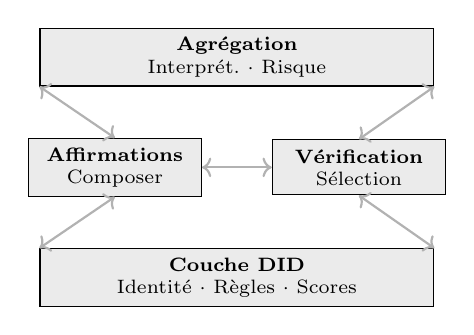
\begin{tikzpicture}[
    layer/.style={draw, minimum height=0.7cm, align=center, font=\scriptsize, fill=black!8},
    arr/.style={<->, thick, gray!60}
]
\node[layer, minimum width=5cm] (agg) at (0,2.8) {\textbf{Agrégation}\\Interprét.\ $\cdot$ Risque};
\node[layer, minimum width=2.2cm] (claim) at (-1.55,1.4) {\textbf{Affirmations}\\Composer};
\node[layer, minimum width=2.2cm] (verif) at (1.55,1.4) {\textbf{Vérification}\\Sélection};
\node[layer, minimum width=5cm] (did) at (0,0) {\textbf{Couche DID}\\Identité $\cdot$ Règles $\cdot$ Scores};

\draw[arr] (agg.south west) -- (claim.north);
\draw[arr] (agg.south east) -- (verif.north);
\draw[arr] (claim.east) -- (verif.west);
\draw[arr] (claim.south) -- (did.north west);
\draw[arr] (verif.south) -- (did.north east);
\end{tikzpicture}
\caption{Architecture à quatre couches du RSN.}
\label{fig:architecture}
\end{figure}

\subsection{Rôles des participants}

Une transaction de vérification implique jusqu'à six rôles DID distincts (Fig.~\ref{fig:roles}) : l'\textbf{Émetteur} ($DID_I$, crée et soumet l'affirmation), le \textbf{Sujet} ($DID_S$, le DID sur lequel porte l'affirmation---peut coïncider avec l'Émetteur), l'\textbf{Autorité} ($DID_A$, cautionne l'affirmation contre des honoraires ; peut aussi offrir des services de témoin---\emph{optionnel}), le \textbf{Témoin} ($DID_{W_{1..n}}$, contrôleur incognito de l'honnêteté du vérificateur via des codes de défi---\emph{optionnel}), le \textbf{Vérificateur} ($DID_V$, sélectionné algorithmiquement pour publier l'affirmation), et le \textbf{RSN} (le réseau où les affirmations vérifiées sont publiées). Tout rôle peut être délégué à un autre DID (Section~7.4). Une Autorité regroupe couramment la caution et les services de témoin, mais les deux fonctions sont logiquement indépendantes.

\begin{figure}[ht]
\centering
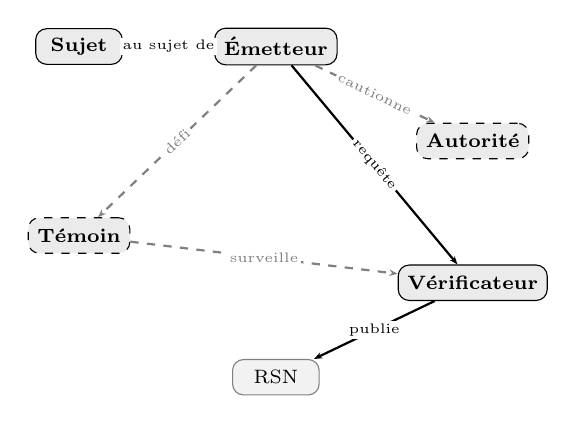
\begin{tikzpicture}[
    role/.style={draw, rounded corners, minimum width=1.1cm, minimum height=0.45cm, align=center, font=\scriptsize, fill=black!8},
    opt/.style={draw, rounded corners, minimum width=1.1cm, minimum height=0.45cm, align=center, font=\scriptsize, fill=black!8, dashed},
    arr/.style={-{Stealth[length=3pt]}, thick},
    oarr/.style={-{Stealth[length=3pt]}, thick, dashed, gray},
    lbl/.style={font=\tiny, fill=white, inner sep=1pt}
]
\node[role] (I) at (0,2.4) {\textbf{Émetteur}};
\node[role] (S) at (-2.5,2.4) {\textbf{Sujet}};
\node[opt] (A) at (2.5,1.2) {\textbf{Autorité}};
\node[opt] (W) at (-2.5,0) {\textbf{Témoin}};
\node[role] (V) at (2.5,-0.6) {\textbf{Vérificateur}};
\node[role, fill=black!5, draw=gray] (N) at (0,-1.8) {RSN};

\draw[arr] (I) -- node[lbl] {au sujet de} (S);
\draw[oarr] (I) -- node[lbl,sloped] {cautionne} (A);
\draw[oarr] (I) -- node[lbl,sloped] {défi} (W);
\draw[arr] (I) -- node[lbl,sloped] {requête} (V);
\draw[oarr] (W) -- node[lbl] {surveille} (V);
\draw[arr] (V) -- node[lbl] {publie} (N);
\end{tikzpicture}
\caption{Rôles DID dans une transaction de vérification. Pointillés = optionnel (Autorité, Témoin).}
\label{fig:roles}
\end{figure}

\subsection{Incorruptibilité : quatre forces}

L'incorruptibilité du RSN ne découle pas d'un mécanisme unique mais de quatre forces concurrentes. Aucune ne suffit à elle seule ; seule leur combinaison rend une tentative de corruption économiquement irrationnelle.

\textbf{Cible imprévisible.} Le vérificateur de chaque affirmation est sélectionné de façon non déterministe par hachage cohérent (Section~5.3). Un attaquant ne peut pas cibler à l'avance un vérificateur précis pour le corrompre, car l'identité du vérificateur est une fonction du contenu de l'affirmation et des itérations précédentes, et non du choix de l'émetteur.

\textbf{Levier réputationnel---lente montée, chute rapide.} La réputation ne peut être acquise que progressivement, par un comportement constant et soutenu. Elle peut toutefois être perdue de façon catastrophique par une seule caution frauduleuse (Section~6.2). Cette asymétrie signifie que des années de réputation accumulée peuvent être détruites par une seule caution malhonnête ; la stratégie optimale reste de rejeter les affirmations suspectes.

\textbf{Promesse publique.} Chaque Détenteur de DID déclare publiquement sa politique---un ensemble de règles lisibles par machine qu'il s'engage à suivre. Toute divergence entre la déclaration et le comportement réel est détectable et tarifée comme une faute réputationnelle plus grave que la violation sous-jacente (Section~7.3). L'hypocrisie est donc plus coûteuse que la malhonnêteté directe.

\textbf{Asymétrie du coût d'attaque du maillage.} Le coût de la censure ou de la déstabilisation du réseau croît de façon non linéaire avec la taille et la densité du réseau, tandis que le coût de sa tolérance reste constant. Pour que la censure soit rentable, un acteur centralisé devrait l'appliquer à l'ensemble du réseau---exigeant des mesures disproportionnées par rapport à tout bénéfice concevable (Section~10).

% ============================================================
% 4. DECENTRALIZED IDENTITY MODEL
% ============================================================
\section{Modèle d'identité décentralisée}

\subsection{DID à propriétés particulières}

Le RSN étend la spécification W3C DID Core~\cite{did2022} avec : des \textbf{Règles déclarées} (engagements comportementaux lisibles par machine), des \textbf{Métadonnées de réputation} (score comportemental agrégé) et un \textbf{Routage réseau} (passerelle onion mutable, distincte de la position stable sur l'anneau).

\subsection{Cycle de vie d'une affirmation}

Une affirmation traverse six étapes (Fig.~\ref{fig:lifecycle}) : composition, caution optionnelle par une autorité, sélection du vérificateur par hachage cohérent, décision de vérification (acceptation ou rejet avec itération), publication et mise à jour de la réputation de toutes les parties.

\begin{figure}[ht]
\centering
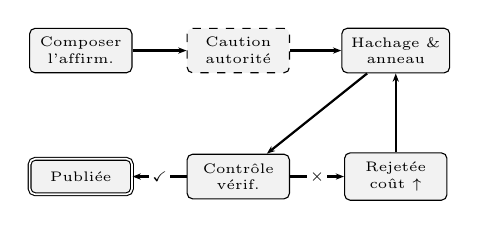
\begin{tikzpicture}[
    stp/.style={draw, rounded corners=2pt, minimum width=1.3cm, minimum height=0.45cm, align=center, font=\tiny, fill=black!5},
    arr/.style={-{Stealth[length=3pt]}, thick},
    lbl/.style={font=\tiny, fill=white, inner sep=1pt}
]
\node[stp] (comp) at (0,0) {Composer\\l'affirm.};
\node[stp, dashed] (auth) at (2.0,0) {Caution\\autorité};
\node[stp] (hash) at (4.0,0) {Hachage \&\\anneau};
\node[stp] (ver) at (2.0,-1.6) {Contrôle\\vérif.};
\node[stp, double] (pub) at (0,-1.6) {Publiée};
\node[stp] (rej) at (4.0,-1.6) {Rejetée\\coût $\uparrow$};

\draw[arr] (comp) -- (auth);
\draw[arr] (auth) -- (hash);
\draw[arr] (hash) -- (ver);
\draw[arr] (ver) -- node[lbl] {\checkmark} (pub);
\draw[arr] (ver) -- node[lbl] {$\times$} (rej);
\draw[arr] (rej) -- ++(0,0.8) -| (hash);
\end{tikzpicture}
\caption{Cycle de vie d'une affirmation avec boucle d'itération.}
\label{fig:lifecycle}
\end{figure}

\subsection{Relation avec W3C DID Core}

Le modèle d'identité du RSN est un sur-ensemble strict de la spécification W3C DID Core~\cite{did2022}. Tous les DID du RSN sont des DID W3C valides. Les extensions spécifiques au RSN sont encodées comme propriétés de document DID définies dans une spécification dédiée de méthode DID, compatible avec les infrastructures existantes telles qu'ION~\cite{buchner2021} et Ceramic~\cite{ceramic2023}.

% ============================================================
% 5. VERIFICATION AND PROPAGATION
% ============================================================
\section{Vérification et propagation de l'information}

\subsection{Coût de l'entrée d'information}

Le principe économique central du RSN est l'asymétrie entre la lecture et l'écriture. La lecture des données de réputation tend vers un coût marginal nul pour les participants qui font partie du réseau DID et disposent d'un accès proportionné à leur réputation---les nouveaux venus doivent progressivement mériter un accès plus large (voir anti-parasitage). L'écriture---comprise comme la matérialisation durable de la réputation dans le réseau, et non comme un acte technique ponctuel---exige un investissement cumulatif vérifiable selon trois dimensions : le \textbf{temps} (des années de vie consacrées à un comportement constant, à des engagements tenus et à des relations cultivées), l'\textbf{énergie} (l'effort investi dans des relations honnêtes, le soin des partenariats et une fiabilité de long terme) et l'\textbf{argent} (l'investissement dans son propre nom---développement professionnel, qualité de son travail, réparation des préjudices causés). La réputation ne peut pas s'acheter instantanément---elle est le résultat d'une accumulation de toute une vie que le système se contente de rendre visible et transférable entre contextes. Les coûts techniques ponctuels du protocole (signatures cryptographiques, honoraires de vérificateur) sont négligeables comparés à cet investissement sous-jacent.

\subsection{Graphe social et profondeur des contacts}

Le RSN est fondamentalement un réseau social : chaque DID ajoute des contacts (d'autres DID) qui autorisent la connexion. Ces contacts ont leurs propres contacts, et ainsi de suite. La recherche algorithmique de vérificateur opère dans une profondeur configurable $h$ de contacts liés (p.\ ex.\ $h=3$ : ses contacts directs, leurs contacts, et les contacts de ces contacts). Cette architecture ne nécessite pas une unique blockchain globale---elle favorise naturellement l'émergence de communautés/grappes avec des chevauchements vers d'autres communautés. Chaque participant DID doit disposer d'une \textbf{politique} publiée---un ensemble de règles lisibles par machine régissant la manière dont les requêtes entrantes sont évaluées. Les violations de politique sont enregistrées dans le réseau comme des artefacts négatifs.

\subsection{Sélection algorithmique des vérificateurs}

Le protocole de vérification emploie le hachage cohérent~\cite{karger1997} (Fig.~\ref{fig:verifier}). La vérification est un service payant : les vérificateurs opèrent contre des honoraires, créant un marché où la concurrence pousse la tarification, la rapidité et la fiabilité.

\textbf{Étape 1.} Le document d'affirmation est concaténé avec le résultat de hachage de l'itération précédente (ou $\varnothing$ à la première itération) puis haché :
\begin{equation}
\text{pos} = f_h(\text{claim} \| \text{prev\_hash})
\label{eq:hash}
\end{equation}

L'algorithme doit inclure le \emph{chemin complet} de toutes les requêtes et réponses précédentes---et non un simple hachage de l'itération précédente. La réponse intégrale de chaque vérificateur (acceptation, rejet, prix indiqué, motif) est ajoutée au document en croissance, vérifiable par des signatures cryptographiques à chaque étape.

\textbf{Étape 2.} Le hachage est projeté sur $N$ positions de l'anneau de hachage cohérent, uniformément réparties (p.\ ex.\ pour $N=4$ : $+0^{\circ}, +90^{\circ}, +180^{\circ}, +270^{\circ}$). À partir de chaque position, une recherche dans le sens horaire sélectionne le DID le plus proche comme candidat vérificateur (Fig.~\ref{fig:multipoint}). $N$ est un paramètre variable qui peut dépendre du pourcentage de DID actuellement actifs, de l'heure de la journée ou de la réactivité historique du réseau.

\textbf{Étape 3.} Le Vérificateur accepte (publie, engageant sa réputation) ou rejette (retour à l'Étape~1 avec le hachage du rejet). Lorsqu'un nœud ne répond pas malgré un statut en ligne déclaré, la requête suivante doit inclure toutes les réponses de l'ensemble des $N$ candidats vérificateurs précédents.

\textbf{Anti-parasitage.} Les DID cibles peuvent fixer des honoraires ou des restrictions d'accès pour les requêtes provenant de nouveaux DID à faible réputation. Ce mécanisme graduel (et non binaire) oblige les nouveaux venus à bâtir une réputation par une activité authentique avant de consommer librement les données d'autrui.

\begin{figure}[ht]
\centering
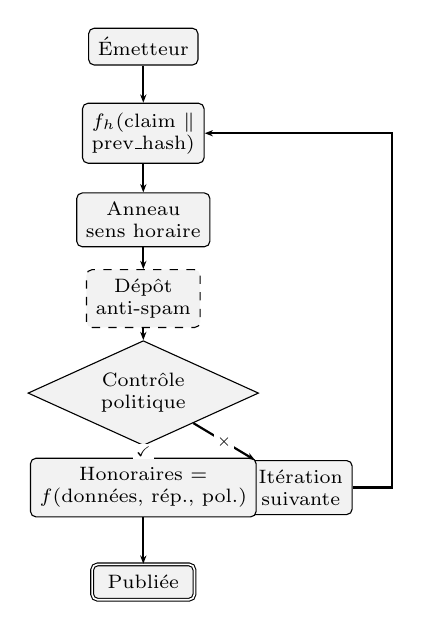
\begin{tikzpicture}[
    box/.style={draw, rounded corners=2pt, minimum width=1.3cm, minimum height=0.45cm, align=center, font=\scriptsize, fill=black!5},
    dec/.style={draw, diamond, aspect=2.2, minimum width=0.9cm, align=center, font=\scriptsize, fill=black!5},
    arr/.style={-{Stealth[length=3pt]}, thick},
    lbl/.style={font=\tiny, fill=white, inner sep=1pt}
]
\node[box] (iss) at (0,0) {Émetteur};
\node[box] (hash) at (0,-1.1) {$f_h$(claim $\|$\\prev\_hash)};
\node[box] (ring) at (0,-2.2) {Anneau\\sens horaire};
\node[box, dashed] (spam) at (0,-3.2) {Dépôt\\anti-spam};
\node[dec] (check) at (0,-4.4) {Contrôle\\politique};
\node[box] (rej) at (2,-5.6) {Itération\\suivante};
\node[box] (fee) at (0,-5.6) {Honoraires =\\$f$(données, rép., pol.)};
\node[box, double] (pub) at (0,-6.8) {Publiée};

\draw[arr] (iss) -- (hash);
\draw[arr] (hash) -- (ring);
\draw[arr] (ring) -- (spam);
\draw[arr] (spam) -- (check);
\draw[arr] (check) -- node[lbl] {$\times$} (rej);
\draw[arr] (check) -- node[lbl] {\checkmark} (fee);
\draw[arr] (fee) -- (pub);
\draw[arr] (rej.east) -- ++(0.5,0) |- (hash.east);
\end{tikzpicture}
\caption{Protocole de sélection des vérificateurs. Le dépôt anti-spam est optionnel et peut être remboursable. Les honoraires finaux ne sont dus qu'en cas d'acceptation.}
\label{fig:verifier}
\end{figure}

Chaque rejet ajoute la réponse intégrale du vérificateur (y compris les motifs et conditions) au document d'affirmation, en élargissant son contenu. À partir du document élargi, un nouveau hachage est calculé de façon non déterministe, projeté sur une position différente de l'anneau et sélectionnant un vérificateur différent. La documentation du chemin complet est obligatoire---l'émetteur ne peut ni prédire ni influencer le vérificateur suivant. Si un vérificateur ignore une requête malgré une politique déclarée compatible, les témoins (le cas échéant) le consignent, et l'émetteur peut joindre les preuves des témoins lors de la publication finale.

\begin{figure}[ht]
\centering
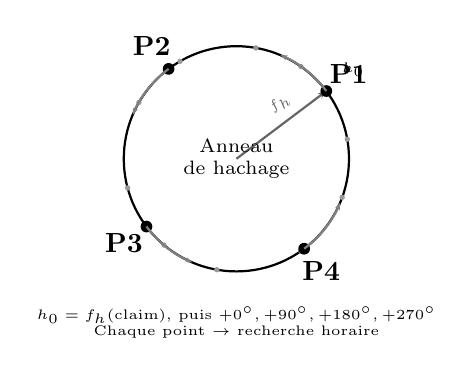
\begin{tikzpicture}[scale=0.65]
% Ring
\draw[thick] (0,0) circle (2.2cm);
% DID nodes on ring
\foreach \a in {10,55,80,120,150,195,230,260,305,340} {
  \fill[black!40] (\a:2.2) circle (1.5pt);
}
% Hash offset arrow pointing to initial position
\draw[-{Stealth[length=3pt]}, thick, black!60] (0,0) -- node[font=\tiny,above,sloped,pos=0.6] {$f_h$} (37:2.2);
\fill[black] (37:2.2) circle (2pt);
\node[font=\tiny,anchor=south west] at (37:2.35) {$h_0$};
% N=4 points offset from h0 by +0, +90, +180, +270
\foreach \offset/\l in {0/P1,90/P2,180/P3,270/P4} {
  \pgfmathsetmacro{\ang}{37+\offset}
  \node[fill=black, circle, inner sep=1.5pt] (p\offset) at (\ang:2.2) {};
  \node[font=\tiny,font=\bfseries] at (\ang:2.75) {\l};
  % clockwise search arc
  \draw[-{Stealth[length=2.5pt]}, thick, gray] (\ang:2.2) arc (\ang:\ang+30:2.2);
}
\node[font=\scriptsize, align=center] at (0,0) {Anneau\\de hachage};
\node[font=\tiny, align=center] at (0,-3.2) {$h_0 = f_h(\text{claim})$, puis $+0^{\circ},+90^{\circ},+180^{\circ},+270^{\circ}$\\Chaque point $\rightarrow$ recherche horaire};
\end{tikzpicture}
\caption{Sélection multipoint ($N{=}4$). Le hachage $h_0$ fixe le décalage ; 4 points uniformément répartis à partir de $h_0$.}
\label{fig:multipoint}
\end{figure}

\subsection{Protocole du témoin}

Le rôle du \textbf{Témoin} fournit une responsabilisation incognito de l'honnêteté du vérificateur au moyen d'un protocole cryptographique de code de défi :

\textbf{Étape W1.} Le demandeur signe la requête de vérification et l'envoie à $N_w$ témoins---des contacts du réseau social du demandeur, ou des prestataires spécialisés de service de témoin opérant contre des honoraires.

\textbf{Étape W2.} Chaque témoin $w_i$ signe l'intégralité de la requête signée, conserve la signature originale $\sigma_i$ et calcule un code de défi $c_i = h(\sigma_i)$. Le code de défi est ajouté à la requête.

\textbf{Étape W3.} La requête, portant désormais $N_w$ codes de défi, est envoyée au vérificateur. Le vérificateur observe les codes mais \emph{ne peut pas déterminer} qui sont les témoins ni si les codes correspondent à de vraies signatures.

\textbf{Étape W4 (vérificateur honnête).} Si le vérificateur répond conformément à sa politique déclarée, les codes de défi restent opaques. Les témoins ne sont jamais révélés. Aucune donnée supplémentaire n'est publiée.

\textbf{Étape W5 (violation de politique).} Si le vérificateur enfreint sa politique (ignore la requête, répond de façon incohérente), le demandeur détient les signatures originales $\sigma_i$ des témoins. Celles-ci peuvent être publiées comme données d'accompagnement : quiconque peut vérifier que $c_i = h(\sigma_i)$, prouvant que le témoin était présent. Le demandeur peut publier de façon indépendante---le vérificateur a déjà signé les codes de défi dans sa réponse.

\textbf{La propriété de bluff.} Le demandeur peut substituer des valeurs aléatoires à certains ou à tous les codes de défi. Le vérificateur ne peut pas distinguer les codes authentiques (adossés à des autorités de haute réputation) du bruit. Cette \emph{incertitude} est le mécanisme d'application : chaque requête porte le risque qu'une autorité respectée observe incognito. Le coût du maintien de cette pression est proche de zéro (générer des nombres aléatoires), tandis que le coût potentiel de la malhonnêteté pour le vérificateur est catastrophique. Le comportement honnête est incité même en l'absence de témoins réels.

\textbf{L'Autorité comme témoin.} Une Autorité qui cautionne une affirmation peut regrouper les services de témoin : «~Je cautionne votre affirmation et je fais office de témoin incognito pendant la vérification.~» C'est un modèle économique naturel---l'Autorité dispose déjà du contexte. Les deux rôles restent toutefois logiquement indépendants.

\subsection{Principe du radicalisme coûteux}

Trois canaux de coûts se cumulent simultanément (Fig.~\ref{fig:radicalism}) :

\textbf{Canal 1 : coût d'itération.} Chaque rejet impose une nouvelle itération qui consomme du temps et des ressources. Croissance linéaire.

\textbf{Canal 2 : gonflement du document.} Chaque itération ajoute la réponse intégrale du vérificateur au document d'affirmation. La croissance est linéaire, mais avec un décalage de base : la charge utile initiale (contenu de l'affirmation, caution de l'autorité, signatures cryptographiques) possède déjà une taille non triviale $B_0$. Taille totale après $k$ itérations : $S(k) = B_0 + k \cdot \Delta$, où $\Delta$ est la taille moyenne d'une réponse.

\textbf{Canal 3 : prime de risque du vérificateur.} Le risque est subjectif. Le vérificateur évalue si les politiques déclarées du DID demandeur entrent en conflit avec ses propres intérêts commerciaux, sociaux ou politiques. La prime peut croître de façon exponentielle avec la distance perçue à l'«~idéal~» du vérificateur : $P(d) = \alpha \cdot e^{\beta d}$, où $d$ est la métrique de distance subjective du vérificateur. Au-delà d'une frontière personnelle infranchissable, le vérificateur peut refuser purement et simplement.

\begin{figure}[ht]
\centering
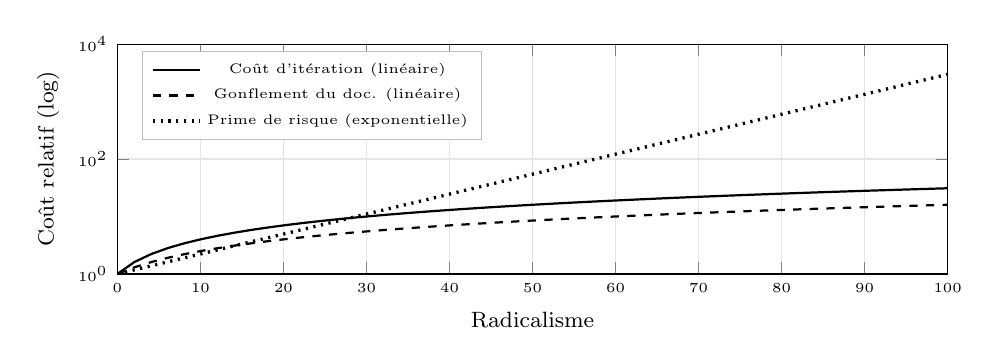
\begin{tikzpicture}
\begin{axis}[
    width=\columnwidth,
    height=4.5cm,
    xlabel={\footnotesize Radicalisme},
    ylabel={\footnotesize Coût relatif (log)},
    ymode=log,
    xmin=0, xmax=100,
    ymin=1, ymax=10000,
    grid=major,
    grid style={gray!20},
    legend style={at={(0.03,0.97)},anchor=north west,font=\tiny,draw=gray!50},
    tick label style={font=\tiny},
    label style={font=\footnotesize},
]
\addplot[black, thick, domain=0:100, samples=50] {1 + 0.3*x};
\addlegendentry{Coût d'itération (linéaire)}
\addplot[black, thick, dashed, domain=0:100, samples=50] {1 + 0.15*x};
\addlegendentry{Gonflement du doc. (linéaire)}
\addplot[black, thick, dotted, line width=1.2pt, domain=0:100, samples=100] {exp(0.08*x)};
\addlegendentry{Prime de risque (exponentielle)}
\end{axis}
\end{tikzpicture}
\caption{Escalade des coûts sur trois canaux. La prime de risque domine à haut radicalisme.}
\label{fig:radicalism}
\end{figure}

Fait crucial, ce n'est pas de la censure. Aucune affirmation n'est interdite. Le système tarifie le risque (Table~\ref{tab:costs}).

\begin{table}[ht]
\centering
\caption{Comparaison des coûts par type d'affirmation.}
\label{tab:costs}
\footnotesize
\begin{tabular}{@{}lcccc@{}}
\toprule
\textbf{Type} & \textbf{Itér.} & \textbf{Doc} & \textbf{Honor.} & \textbf{Total} \\
\midrule
Crédible & $k_{\min}$ & $B_0$ & $P_{\min}$ & Faible \\
Controversée & $k_{\text{med}}$ & $B_0{+}k\Delta$ & $\alpha e^{\beta d}$ & Modéré \\
Radicale & $k_{\max}$ & $\gg B_0$ & $\gg P_{\min}$ & Très élevé \\
Frauduleuse & $\to\infty$ & --- & --- & Impubliable \\
\bottomrule
\end{tabular}
\end{table}

% ============================================================
% 6. REPUTATION AND RISK
% ============================================================
\section{Réputation et évaluation du risque}

\subsection{Modèle d'accumulation de la réputation}

La réputation présente trois propriétés : une \textbf{accumulation lente} (croissance progressive par un comportement constant), une \textbf{destruction rapide} (une seule fraude peut réduire le score de façon catastrophique) et une \textbf{évaluation individuelle} (chaque partie consommatrice peut appliquer sa propre fonction d'agrégation).

\subsection{Autorités réputées}

Une Autorité réputée examine les affirmations et, si elle est convaincue, les contresigne---engageant sa propre réputation (Fig.~\ref{fig:authority}). L'asymétrie est intentionnelle : gagner de la réputation est lent (incrément $+\delta$ par caution honnête), tandis que la perdre est catastrophique ($-\Delta \gg \delta$ par caution mensongère ; à titre d'illustration, p.\ ex.\ $+2\%$ contre $-70\%$). La stratégie optimale est toujours de rejeter les affirmations suspectes. Les valeurs précises de $\delta$ et $\Delta$ sont des paramètres du système.

\begin{figure}[ht]
\centering
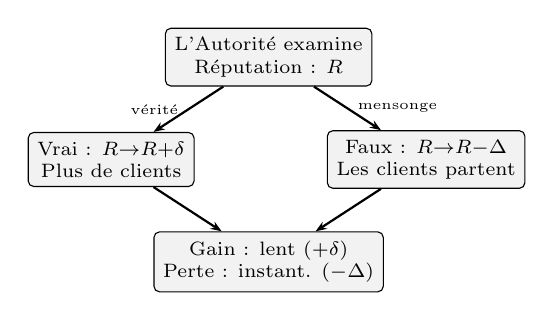
\begin{tikzpicture}[
    box/.style={draw, rounded corners=2pt, minimum width=2cm, minimum height=0.6cm, align=center, font=\scriptsize, fill=black!5},
    arr/.style={-{Stealth[length=4pt]}, thick}
]
\node[box] (exam) at (0,0) {L'Autorité examine\\Réputation : $R$};
\node[box] (true) at (-2,-1.3) {Vrai : $R{\to}R{+}\delta$\\Plus de clients};
\node[box] (false) at (2,-1.3) {Faux : $R{\to}R{-}\Delta$\\Les clients partent};
\node[box] (insight) at (0,-2.6) {Gain : lent ($+\delta$)\\Perte : instant. ($-\Delta$)};

\draw[arr] (exam) -- node[left,font=\tiny] {vérité} (true);
\draw[arr] (exam) -- node[right,font=\tiny] {mensonge} (false);
\draw[arr] (true) -- (insight);
\draw[arr] (false) -- (insight);
\end{tikzpicture}
\caption{Autorité réputée---incitations asymétriques.}
\label{fig:authority}
\end{figure}

\subsection{Réputation multidimensionnelle}

La réputation n'est pas un scalaire mais un vecteur selon plusieurs dimensions : fiabilité financière, intégrité personnelle, compétence professionnelle, engagement civique, et d'autres (Fig.~\ref{fig:reputation-radar}). Différents prestataires d'évaluation projettent ce vecteur différemment selon le contexte---un prêteur privilégie la fiabilité financière, un employeur la compétence professionnelle, un voisin le comportement civique. Il n'existe pas de score de réputation «~correct~» unique ; seulement des perspectives.

\begin{figure}[ht]
\centering
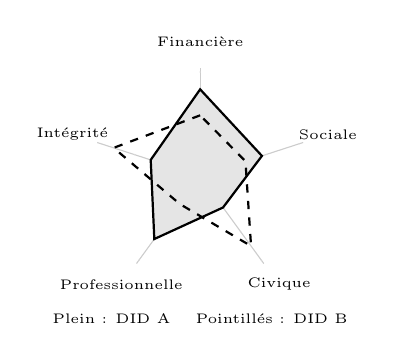
\begin{tikzpicture}[scale=0.55]
\foreach \a/\l in {90/Financière,162/Intégrité,234/Professionnelle,306/Civique,18/Sociale} {
  \draw[gray!40] (0,0) -- (\a:2.5);
  \node[font=\tiny, align=center] at (\a:3.1) {\l};
  \foreach \r in {0.8,1.6,2.4} {
    \fill[black!15] (\a:\r) circle (0.5pt);
  }
}
\draw[thick, fill=black!10] (90:2.0) -- (162:1.2) -- (234:1.8) -- (306:0.9) -- (18:1.5) -- cycle;
\draw[thick, dashed] (90:1.4) -- (162:2.1) -- (234:0.8) -- (306:2.0) -- (18:1.1) -- cycle;
\node[font=\tiny] at (0,-3.3) {Plein : DID A \quad Pointillés : DID B};
\end{tikzpicture}
\caption{Vecteurs de réputation multidimensionnels. Différents DID présentent des profils différents selon les dimensions.}
\label{fig:reputation-radar}
\end{figure}

\subsection{Évaluation démocratisée du risque}

Le RSN démocratise l'évaluation systématique du risque---une capacité aujourd'hui concentrée dans les institutions financières mais applicable bien au-delà de la banque. Les conglomérats industriels évaluant la fiabilité de leurs fournisseurs, les compagnies d'assurance tarifant le risque comportemental, la diligence raisonnable lors des fusions et acquisitions, l'estimation de la durée de vie des équipements dans l'industrie---partout où le risque de contrepartie doit être évalué, le RSN fournit une alternative décentralisée et pilotée par le marché. Un marché de services d'interprétation traduit les données brutes de réputation multidimensionnelle en synthèses exploitables, rendant l'évaluation des contreparties accessible à tout participant à un coût marginal.

% ============================================================
% 7. CONSENSUS AND DISPUTE RESOLUTION
% ============================================================
\section{Consensus et résolution des litiges}

\subsection{Modèle de justice décentralisée}

Le RSN reformule la justice comme un problème de négociation bilatérale. La menace d'une atteinte permanente et vérifiable à la réputation est un moyen de dissuasion plus efficace que des procédures judiciaires que la partie lésée ne peut se permettre.

\subsection{Consensus émergent}

Chaque participant maintient un seuil personnel de satisfaction. Le consensus agrégé du réseau émerge comme la moyenne statistique de milliers de négociations bilatérales (Fig.~\ref{fig:consensus}). Une réponse très supérieure au consensus (barbare) est coûteuse à publier. Une réponse proche du consensus (proportionnée) est bon marché. Le consensus n'est pas une règle---c'est un signal de prix.

\begin{figure}[ht]
\centering
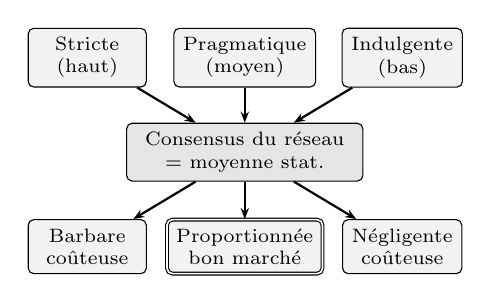
\begin{tikzpicture}[
    person/.style={draw, rounded corners=2pt, minimum width=1.5cm, minimum height=0.5cm, align=center, font=\scriptsize, fill=black!5},
    arr/.style={-{Stealth[length=4pt]}, thick}
]
\node[person] (a) at (-2,0) {Stricte\\(haut)};
\node[person] (b) at (0,0) {Pragmatique\\(moyen)};
\node[person] (c) at (2,0) {Indulgente\\(bas)};
\node[person, fill=black!10, minimum width=3cm] (cons) at (0,-1.2) {Consensus du réseau\\= moyenne stat.};
\node[person] (exp) at (-2,-2.4) {Barbare\\coûteuse};
\node[person, double] (prop) at (0,-2.4) {Proportionnée\\bon marché};
\node[person] (neg) at (2,-2.4) {Négligente\\coûteuse};

\draw[arr] (a) -- (cons);
\draw[arr] (b) -- (cons);
\draw[arr] (c) -- (cons);
\draw[arr] (cons) -- (exp);
\draw[arr] (cons) -- (prop);
\draw[arr] (cons) -- (neg);
\end{tikzpicture}
\caption{Consensus émergent à partir des seuils individuels de satisfaction.}
\label{fig:consensus}
\end{figure}

\subsection{Calibrage de la sanction}

Chaque Détenteur de DID déclare publiquement ses réponses à des catégories spécifiques de fautes. Les déclarations disproportionnellement sévères ou clémentes attirent des signaux de réputation négatifs. Les déclarations proportionnées sont acceptées sans friction---un système de sanction auto-calibrant.

Les déclarations de consensus sont elles-mêmes soumises à la détection d'hypocrisie : s'engager déclarativement sur une position de consensus tout en se comportant de façon incohérente constitue une faute réputationnelle plus grave que l'écart sous-jacent, car cela démontre une tromperie intentionnelle.

\subsection{Délégation}

Toutes les activités au sein d'un DID---à une exception près---peuvent être déléguées à un autre DID. \textbf{Le rôle de Sujet---le DID dont l'affirmation décrit le comportement---ne peut pas être délégué ; il est lié de façon non transférable au détenteur d'identité auquel l'affirmation se rapporte.} Les autres rôles actifs---Émetteur, Autorité, Témoin, Vérificateur---peuvent être transférés à un DID délégué désigné, que ce soit pour la vérification, la soumission d'affirmations, la participation au consensus ou la résolution de litiges. La délégation est révocable à tout moment. Cela permet la spécialisation (p.\ ex.\ des services professionnels de vérification) tandis que le Détenteur conserve le contrôle et la responsabilité ultimes. La délégation s'applique à l'ensemble du système et est essentielle à l'évolutivité.

\subsection{De la morale individuelle au contrat social émergent}

La politique déclarée de chaque DID représente une formalisation de la morale individuelle : ce que le Détenteur considère comme acceptable, la manière dont il répond à des comportements précis, ce qu'il exige de ses contreparties. Ces politiques ne sont pas imposées par un concepteur de système---elles sont choisies par chaque participant et exprimées sous forme lisible par machine.

Cette formalisation rend possible une émergence en trois étapes. D'abord, la morale individuelle est encodée comme \textbf{politique}---un ensemble de règles déclarées, de seuils et de fonctions de réponse que le DID s'engage à suivre. Ensuite, l'agrégat de toutes les politiques du réseau produit une \textbf{éthique émergente}---des normes statistiquement observables qu'aucun participant n'a conçues mais qui naissent de l'interaction de milliers de positions morales individuelles~\cite{durkheim1893}. Enfin, cette éthique émergente, exprimée comme des normes comportementales partagées appliquées par des signaux de prix bilatéraux, constitue un \textbf{contrat social mesurable}---non pas une construction théorique que personne n'a signée~\cite{rawls1971}, mais un ensemble de règles empiriquement observable adossé à des comportements réels.

Ce processus reflète les conclusions de la théorie des fondements moraux~\cite{haidt2012} : la morale humaine est intuitive, plurielle et culturellement variable. Le RSN n'exige pas de consensus moral en entrée ; il produit un consensus comportemental en sortie. Le contrat social qui en résulte n'est pas statique---il évolue à mesure que les participants rejoignent, quittent et ajustent leurs politiques en réponse à la rétroaction du réseau. Contrairement à la théorie classique du contrat social, ce contrat est révocable, observable et applicable sans souverain.

% ============================================================
% 8. ECONOMIC MODEL
% ============================================================
\section{Modèle économique}

Les sections précédentes ont décrit un outil---les mécanismes de vérification du RSN, sa structure de coûts et son consensus émergent. Cette section décrit une méthodologie pour appliquer cet outil à la transition fiscale et de gouvernance. L'outil est polyvalent ; la méthodologie ci-dessous n'est qu'une application possible.

\subsection{Structure des incitations}

La réputation en tant que capital crée des incitations directes à un comportement honnête. En fonctionnement normal, les participants bâtissent leur réputation naturellement par leurs transactions quotidiennes et leurs engagements tenus. La dépense principale porte sur les affirmations \emph{négatives}---consigner un préjudice causé par autrui. Cette asymétrie incite à un comportement utile et fiable : être honnête ne coûte rien de plus, tandis qu'être nuisible crée une trace documentée que d'autres paieront pour conserver. L'hypocrisie---déclarer des règles sans les suivre---est le mode de défaillance le plus coûteux, car elle démontre une tromperie intentionnelle.

\subsection{Système fiscal parallèle}

Trois composantes permettent une pression concurrentielle : (1)~un \textbf{Impôt simple}---un taux proportionnel unique sans exception, initialement légèrement inférieur au taux effectif existant ; (2)~l'\textbf{Enregistrement électronique des dépenses (EED)}---inversant le modèle tchèque EET pour que les citoyens surveillent les dépenses de l'État ; (3)~l'\textbf{Affectation de l'impôt dirigée par le citoyen}---débutant à quelques pour cent la première année et atteignant, au bout d'une décennie, de la dizaine de pour cent à une migration complète vers un système dirigé par le citoyen, selon le rythme d'adoption. Le tempo réel dépend de la vitesse à laquelle émergent des alternatives de libre marché aux services de l'État et de la disposition de l'État à coopérer à la transition ; la fonction du temps n'a pas à être linéaire, et il n'y a aucune raison de fixer une borne supérieure à l'endroit où l'adoption pourra finalement parvenir.

% ============================================================
% 9. MIGRATION PATH
% ============================================================
\section{Voie de migration}

La migration se déroule en trois phases (Fig.~\ref{fig:migration}) : \textbf{Phase~1 : superposition} (le RSN comme couche informationnelle, l'État seul prestataire), \textbf{Phase~2 : concurrence} (le RSN propose des alternatives fonctionnelles, usage à double système) et \textbf{Phase~3 : transition} (le RSN surpasse les équivalents étatiques, migration volontaire). La transition est réversible à chaque étape.

\begin{figure}[ht]
\centering
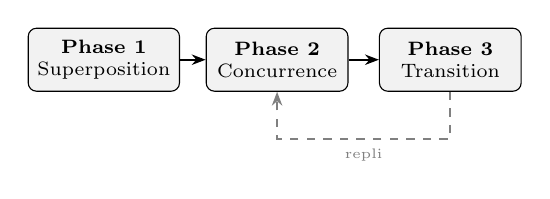
\begin{tikzpicture}[
    phase/.style={draw, rounded corners=3pt, minimum width=1.8cm, minimum height=0.8cm, align=center, font=\scriptsize, fill=black!5},
    arr/.style={-{Stealth[length=5pt]}, thick}
]
\node[phase] (p1) at (0,0) {\textbf{Phase 1}\\Superposition};
\node[phase] (p2) at (2.2,0) {\textbf{Phase 2}\\Concurrence};
\node[phase] (p3) at (4.4,0) {\textbf{Phase 3}\\Transition};

\draw[arr] (p1) -- (p2);
\draw[arr] (p2) -- (p3);
\draw[arr, dashed, gray] (p3.south) -- ++(0,-0.6) -| node[below,font=\tiny,pos=0.25] {repli} (p2.south);
\end{tikzpicture}
\caption{Migration en trois phases---réversible à chaque étape.}
\label{fig:migration}
\end{figure}

Le principal mécanisme de pression est fiscal : lorsque les contribuables conditionnels atteignent une «~minorité économiquement significative $X$~»---un groupe assez important pour que la répression à son encontre cause des dommages économiques non négligeables et que la désobéissance civile devienne une menace crédible---l'État entre en négociation. À titre d'illustration, nous utilisons $X \approx 15\%$ du PIB, mais le seuil réel dépend de l'économie considérée.

% ============================================================
% 10. SECURITY ANALYSIS
% ============================================================
\section{Analyse de sécurité}

Nous considérons cinq catégories d'adversaires : les mauvais acteurs individuels, les groupes organisés, les adversaires corporatifs, les adversaires étatiques et les adversaires au niveau du protocole.

\textbf{Résistance Sybil}~\cite{douceur2002}. Bâtir une réputation exige une interaction soutenue et vérifiable. Le coût d'une attaque Sybil réussie croît linéairement avec le nombre de fausses identités et quadratiquement avec le niveau de réputation visé. Exploiter plusieurs DID en parallèle est possible mais coûteux par conception---chaque identité doit accumuler indépendamment sa réputation par une activité authentique. Dans les sociétés libres, ce coût dissuade les abus occasionnels ; dans les dictatures, les DID parallèles deviennent un outil de survie permettant une résistance cloisonnée, une coordination clandestine et une navigation plus sûre dans le marché noir.

\textbf{Défense contre la collusion.} Les schémas de caution mutuelle au sein de groupes fermés sont détectables par l'analyse du graphe social. Les fonctions d'agrégation de réputation décotent les affirmations provenant de sources étroitement regroupées.

\textbf{Adversaire étatique.} Le routage onion, l'absence d'infrastructure centralisée et la répartition du rôle de Vérificateur sur l'ensemble des participants garantissent que la répression exige des mesures disproportionnées par rapport à tout bénéfice.

\textbf{Vie privée vs.\ responsabilisation.} Le pseudonymat---un terrain intermédiaire entre l'anonymat et la divulgation d'identité---permet aux DID d'accumuler une réputation significative sans révéler l'identité réelle du Détenteur.

% ============================================================
% 11. PRIVACY
% ============================================================
\section{Considérations relatives à la vie privée}

Le modèle de vie privée du RSN repose sur le pseudonymat. Le Détenteur contrôle la divulgation d'identité : minimale (pseudonyme pur), sélective (certains attestations liées) ou complète (identité légale associée). Les affirmations publiées sont permanentes---le système prend en charge la correction contextuelle mais pas l'effacement. Un Détenteur peut abandonner un DID compromis et repartir à zéro, renonçant à la réputation accumulée.

% ============================================================
% 12. RELATED WORK
% ============================================================
\section{Travaux connexes}

La spécification W3C DID Core~\cite{did2022} et le réseau Ceramic~\cite{ceramic2023} fournissent le socle d'identité. EigenTrust~\cite{kamvar2003} a démontré l'agrégation distribuée de réputation sans autorité centrale. Les SBT~\cite{weyl2022} ont introduit des jetons sociaux non transférables. Le RSN s'en distingue par l'accent qu'il met sur le coût économique comme filtre de qualité et par son mécanisme de tarification du radicalisme.

Les DAO~\cite{buterin2014} et le vote quadratique~\cite{buterin2019} ont démontré la faisabilité d'une gouvernance décentralisée. Le RSN dérive son consensus de négociations bilatérales de prix plutôt que du vote.

La proposition s'appuie sur la théorie anarcho-capitaliste~\cite{rothbard1973,hoppe2001} pour la fourniture privée de services mais s'en écarte sous deux aspects critiques : elle est conçue pour les pulsions de rancune et de rétribution plutôt que de présumer la rationalité, et elle propose une transition graduelle plutôt qu'une révolution. Le concept de contrats sociaux émergents a des antécédents dans la théorie de l'ordre spontané de Hayek~\cite{hayek1973}.

\textbf{Anarcho-agorisme.} Le RSN partage un terrain commun important avec la contre-économie agoriste~\cite{konkin2006}---en particulier l'accent mis sur la construction d'institutions parallèles et l'échange volontaire. Cependant, l'agorisme tend à présumer l'intérêt personnel rationnel comme mécanisme de coordination suffisant et manque souvent d'une voie de migration concrète depuis les structures étatiques existantes. Le RSN intègre explicitement des tendances comportementales non rationnelles et fournit un mécanisme de pression fiscale pour une transition graduelle.

\textbf{Méritocratie.} Le RSN pourrait constituer une première description fonctionnelle de la manière dont la méritocratie~\cite{young1958} peut émerger comme propriété systémique plutôt que comme slogan. Les systèmes méritocratiques traditionnels échouent parce qu'ils exigent une autorité centrale pour définir et faire respecter le «~mérite~». Dans le RSN, le mérite émerge des évaluations bilatérales : ceux qui apportent de la valeur accumulent de la réputation ; aucun comité ne décide qui a du mérite.

\textbf{La propriété comme privilège.} Le RSN s'écarte fondamentalement des traitements anarcho-capitalistes et de l'école autrichienne qui considèrent les droits de propriété comme naturels et absolus. Dans le cadre du RSN, la propriété est un \emph{privilège}---une reconnaissance sociale qui peut, dans des cas extrêmes, être retirée par la communauté lorsqu'un participant viole fondamentalement les normes partagées (trahison, refus de défendre la communauté en cas de crise existentielle, exploitation systématique). Il ne s'agit pas d'une expropriation par l'État mais d'un retrait de reconnaissance sociale par le réseau des relations bilatérales.

% ============================================================
% 13. LIMITATIONS
% ============================================================
\section{Discussion et limites}

\textbf{Démarrage à froid.} La valeur du RSN dépend des effets de réseau ; les premiers adoptants font face à une valeur limitée jusqu'à ce que la participation atteigne un seuil. Néanmoins, même dès les premières étapes, le réseau DID sert de source d'information complémentaire utile. On s'attend à ce que l'évaluation précoce de la réputation et l'appréciation des autorités se développent progressivement avec une sophistication croissante.

\textbf{Anti-parasitage et contrôle d'accès.} Les DID cibles peuvent imposer des honoraires graduels et des restrictions d'accès aux requêtes provenant de DID à faible réputation. Ce n'est pas binaire mais une échelle continue : moins un DID demandeur a de réputation, moins il reçoit d'information, plus il attend et plus il paie. Ce mécanisme incite à une participation authentique plutôt qu'à une consommation passive.

\textbf{Inégalité d'accès.} Le coût de publication des affirmations peut filtrer les griefs légitimes des participants économiquement défavorisés. Atténuation : chaque participant sert simultanément de vérificateur potentiel (ou délègue ce rôle) et gagne des honoraires de vérification. Sur un horizon temporel suffisant, un participant non radical devrait tendre vers une neutralité financière---les revenus de vérification compensant approximativement les coûts de publication. C'est une espérance statistique, non une garantie.

\textbf{Inégalité de réputation.} Les premiers adoptants accumulent des avantages susceptibles de créer des barrières pour les arrivants tardifs. Toutefois, l'évaluation de la réputation est réalisée par des prestataires tiers qui peuvent choisir d'atténuer l'avantage du premier arrivé au moyen de leurs algorithmes d'agrégation. Être le premier avec une bonne réputation est un avantage économique comparatif légitime---et c'est voulu.

\textbf{Questions ouvertes.} Les fonctions de coût optimales, les standards d'agrégation, la gouvernance du protocole et l'interaction avec les données de réputation synthétique générées par IA restent des domaines à explorer.

Cet article ne prétend pas que le RSN produira des résultats optimaux en toutes circonstances. Il prétend que le RSN représente une alternative \emph{réalisable}---techniquement implémentable, économiquement autosuffisante et socialement compatible avec les tendances comportementales humaines telles qu'elles sont réellement.

% ============================================================
% 14. CONCLUSION
% ============================================================
\section{Conclusion}

Cet article a présenté le Réseau social de réputation, un protocole décentralisé permettant un échange de réputation pseudonyme et vérifiable. Le Principe du radicalisme coûteux garantit que les affirmations frauduleuses sont écartées par leur prix, sans censure. La voie de migration proposée permet une transition graduelle et réversible depuis les institutions existantes. La conception intègre la nature humaine telle qu'elle est---y compris la mesquinerie, la rancune et le désir de satisfaction punitive---plutôt que d'exiger une transformation idéologique. Le résultat n'est pas l'utopie mais un système où la justice est accessible, où la réputation se mérite et où le coût de la faute est supporté par la partie qui l'a causée.

% ============================================================
% REFERENCES
% ============================================================
\bibliography{references}

\end{document}
